\section{Processamento de Imagens}\label{sec:processamento_imagens}

A partir do  processamento de imagens, é possível identificar a quantidade e classificar o tipo de medicamento no copo. Dessa forma, o processamento de imagens é um método para verificação se a dose medicamentosa, que vai ser entregue ao paciente, está correta, conforme a receita médica.

\subsection{Separação dos comprimidos}

A primeira etapa para extrair dados da imagem é isolar os comprimidos presentes. Para isso, é necessário a conversão da imagem para escala de cinza, facilitando assim na utilização de operações de filtragem na imagem em etapas subsequentes. Para exemplificar a explicação, daqui em diante utiliza-se uma imagem do banco de dados, original na Fig. \ref{fig:proOrig}, e, aplicando a conversão para escala de cinza, temos o resultado na Fig. \ref{fig:proCinza}.

Em seguida, é necessária a detecção das bordas do comprimido. Como as imagens do banco de dados possuem um fundo padronizado, o uso da técnica de limiar é possível. Um resultado possível pode ser observado na Fig. \ref{fig:proLim}. 

O próximo passo é eliminar resíduos da imagem, deixando apenas o contorno do comprimido. Para isso, são realizadas operações de abertura e fechamento, utilizando elementos estruturantes circulares maiores que o resíduo e menores que o comprimido. Com isso, obtemos uma máscara do exemplo utilizado, na Fig. \ref{fig:proMask}.

Por fim, uma técnica de detecção de objetos conectados é aplicada, a qual consegue separar objetos na imagem por meio de observação da vizinhança na imagem. Aplicando essa técnica nos exemplos, temos o resultado nas Fig. \ref{fig:proMask1} e \ref{fig:proMask2}. 

Com a máscara segmentada, é possível separar os comprimidos por meio de uma multiplicação com a imagem original. Com isso, obtemos as Fig. \ref{fig:proPill1} e \ref{fig:proPill2}.

\begin{figure}[H]
        \centering
        \subfloat[][Original]{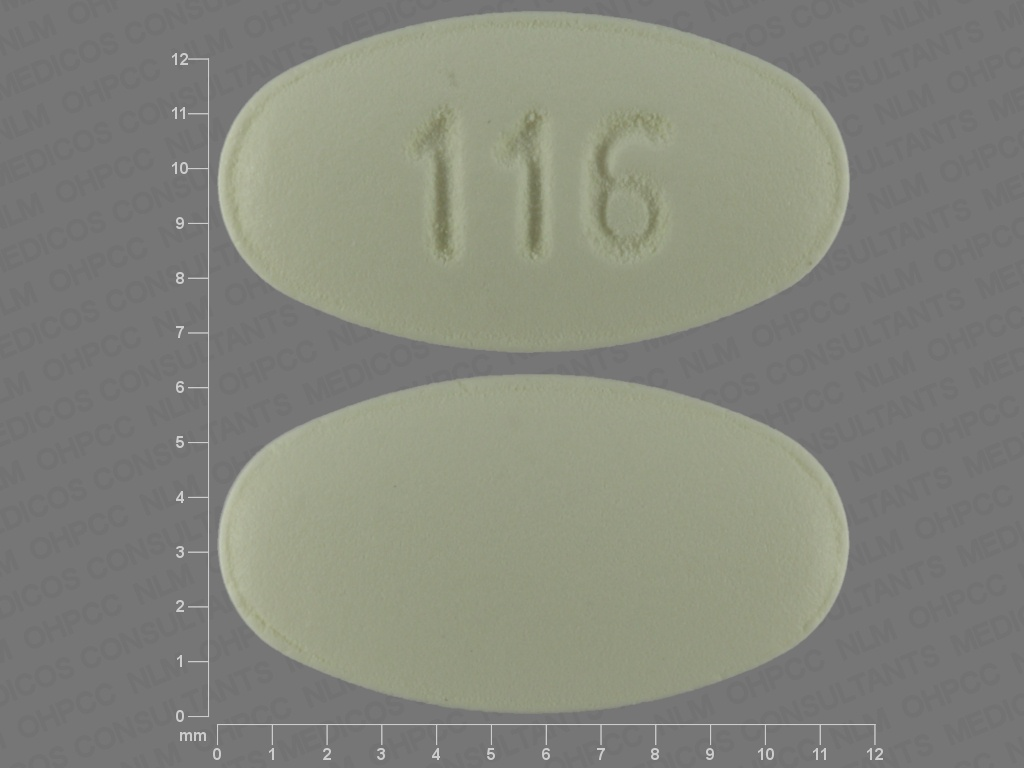
\includegraphics[width=0.25\textwidth]{figuras/eletronica/processamento/original.jpg}\label{fig:proOrig}}
        %\hspace{0.1\textwidth}
        \subfloat[][Escala de cinza]{
        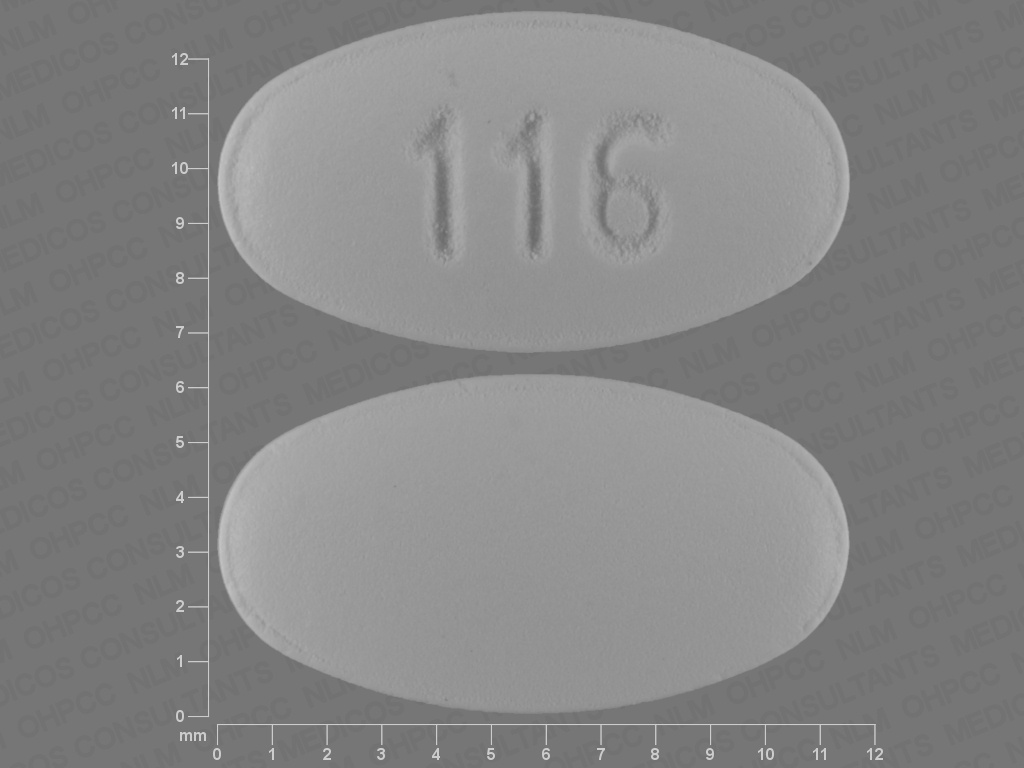
\includegraphics[width=0.25\textwidth]{figuras/eletronica/processamento/cinza.jpg}\label{fig:proCinza}}
        \subfloat[][Limiar]{
        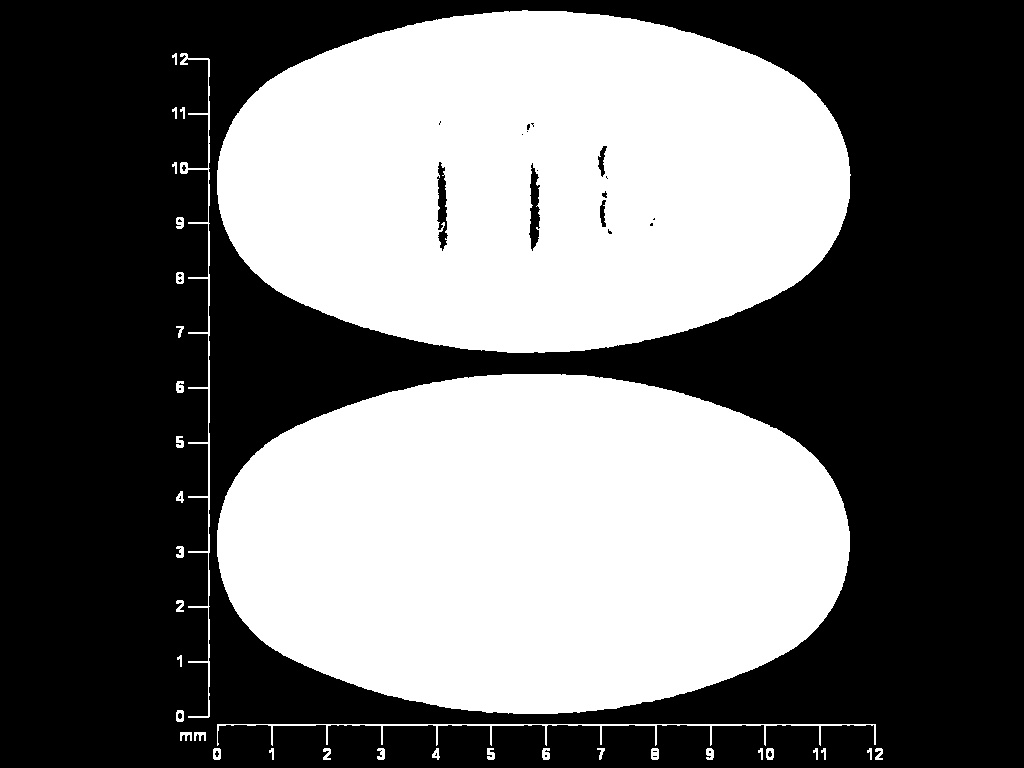
\includegraphics[width=0.25\textwidth]{figuras/eletronica/processamento/limiar.jpg}\label{fig:proLim}}
        
        \subfloat[][Máscara]{
        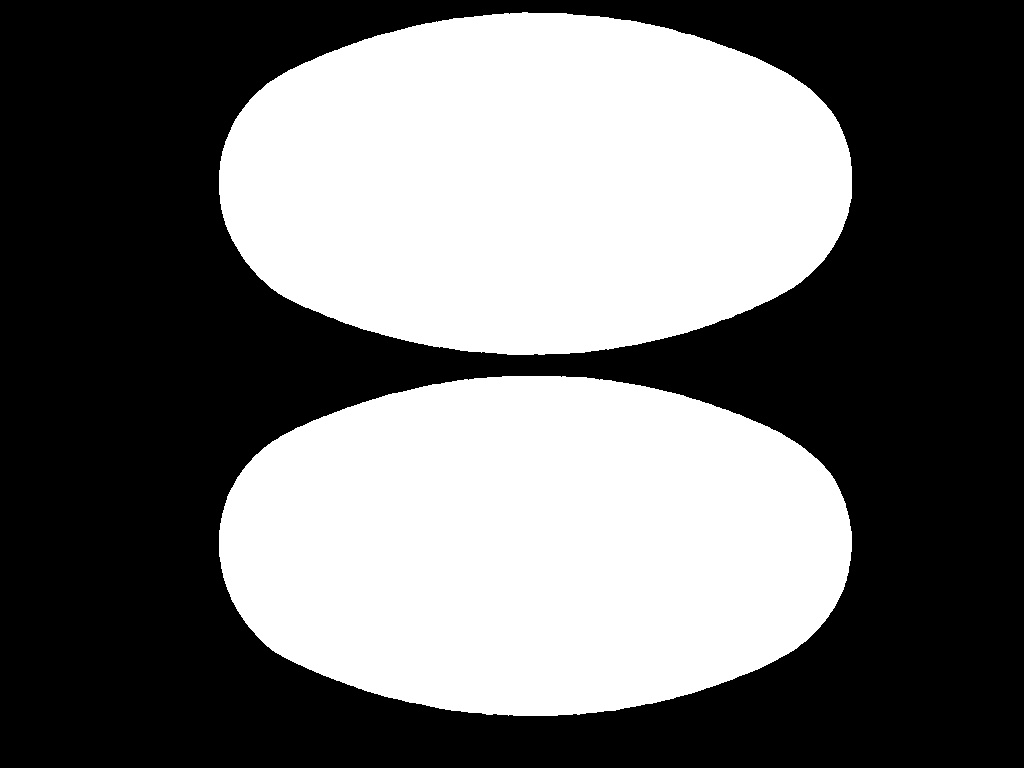
\includegraphics[width=0.25\textwidth]{figuras/eletronica/processamento/mascara.jpg}\label{fig:proMask}}
        \subfloat[][Objeto 1]{
        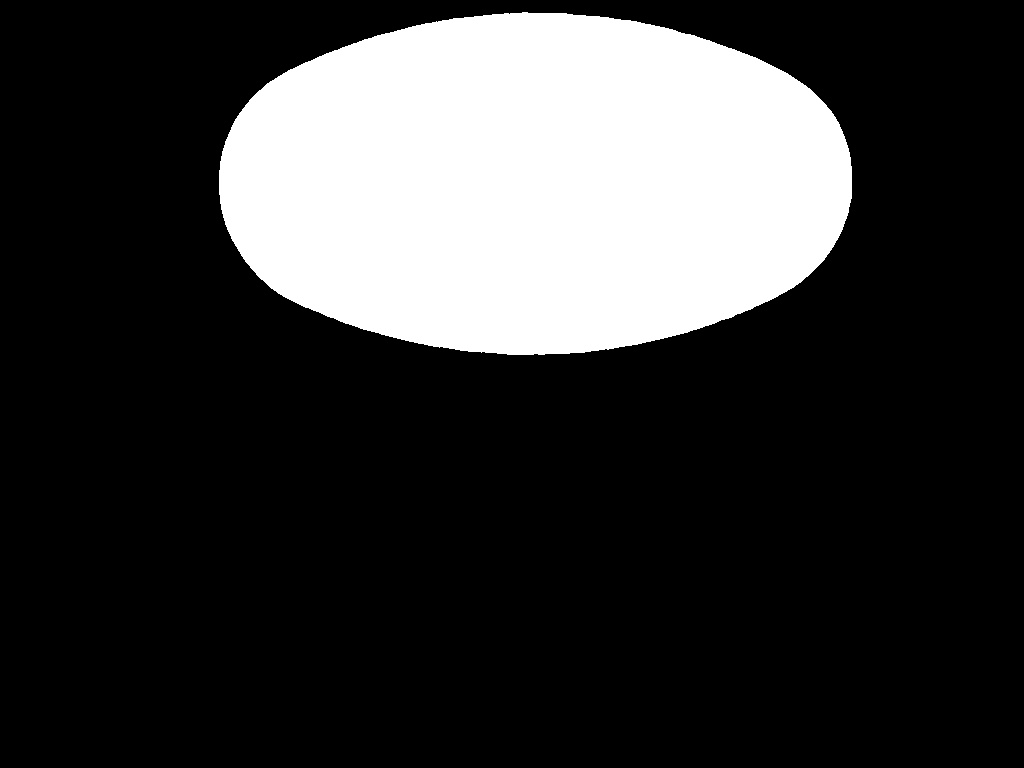
\includegraphics[width=0.25\textwidth]{figuras/eletronica/processamento/mascara1.jpg}\label{fig:proMask1}}
        \subfloat[][Objeto 2]{
        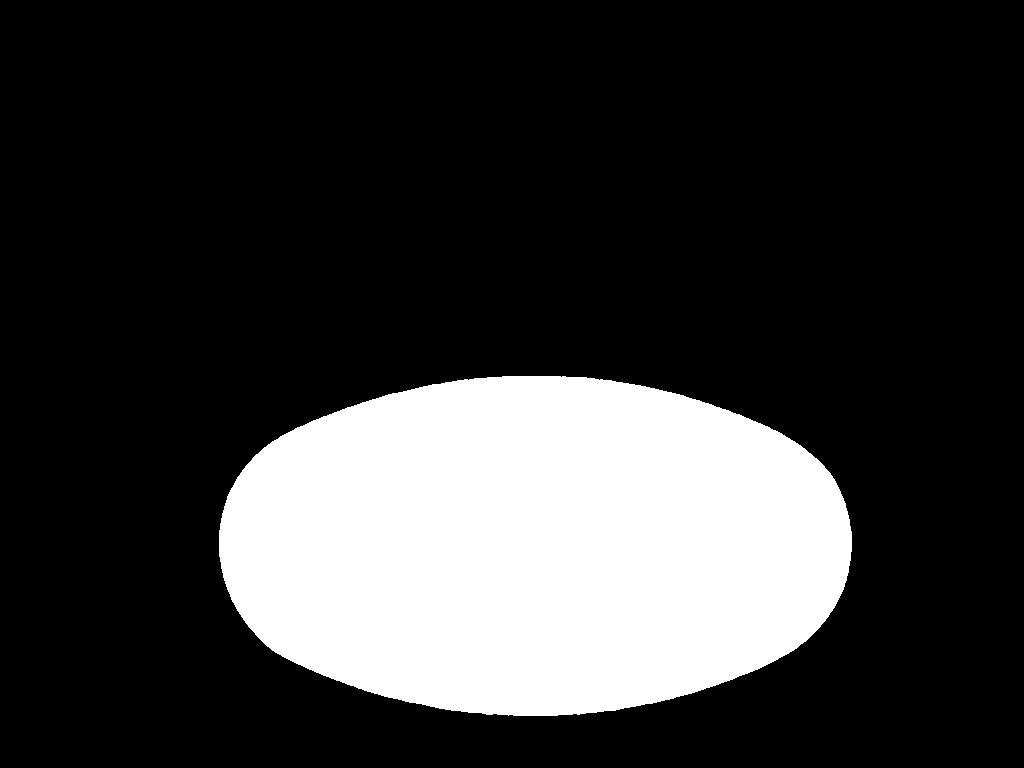
\includegraphics[width=0.25\textwidth]{figuras/eletronica/processamento/mascara2.jpg}\label{fig:proMask2}}
        
        \subfloat[][Comprimido 1]{
        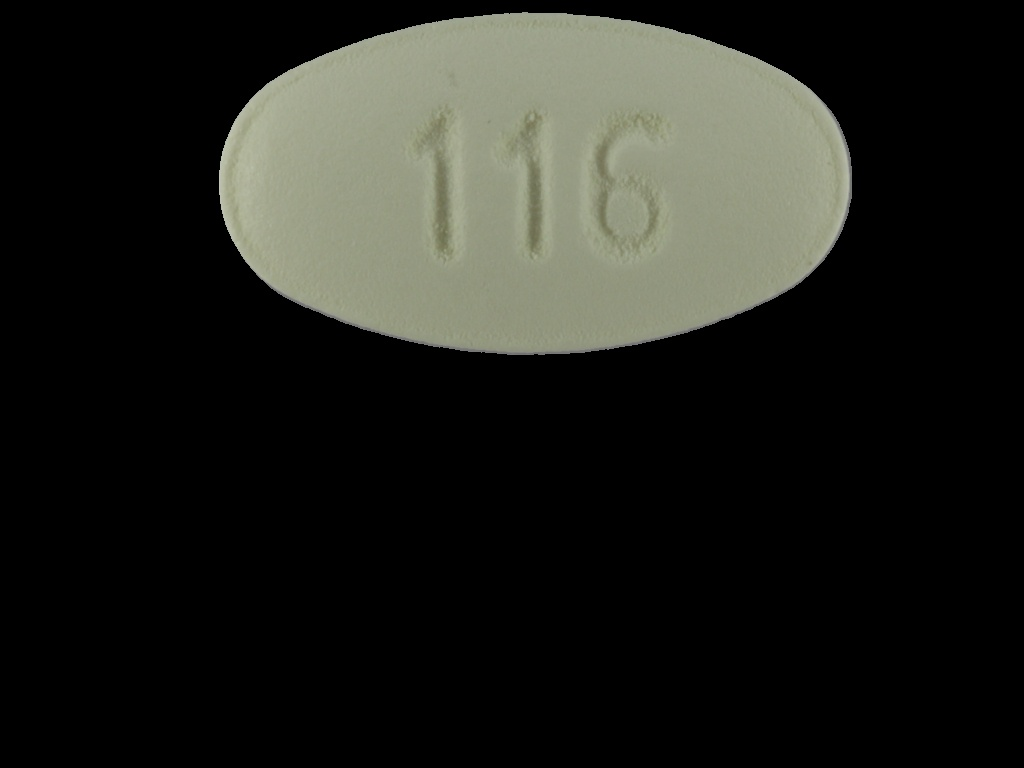
\includegraphics[width=0.25\textwidth]{figuras/eletronica/processamento/pilula1.jpg}\label{fig:proPill1}}
        \subfloat[][Comprimido 2]{
        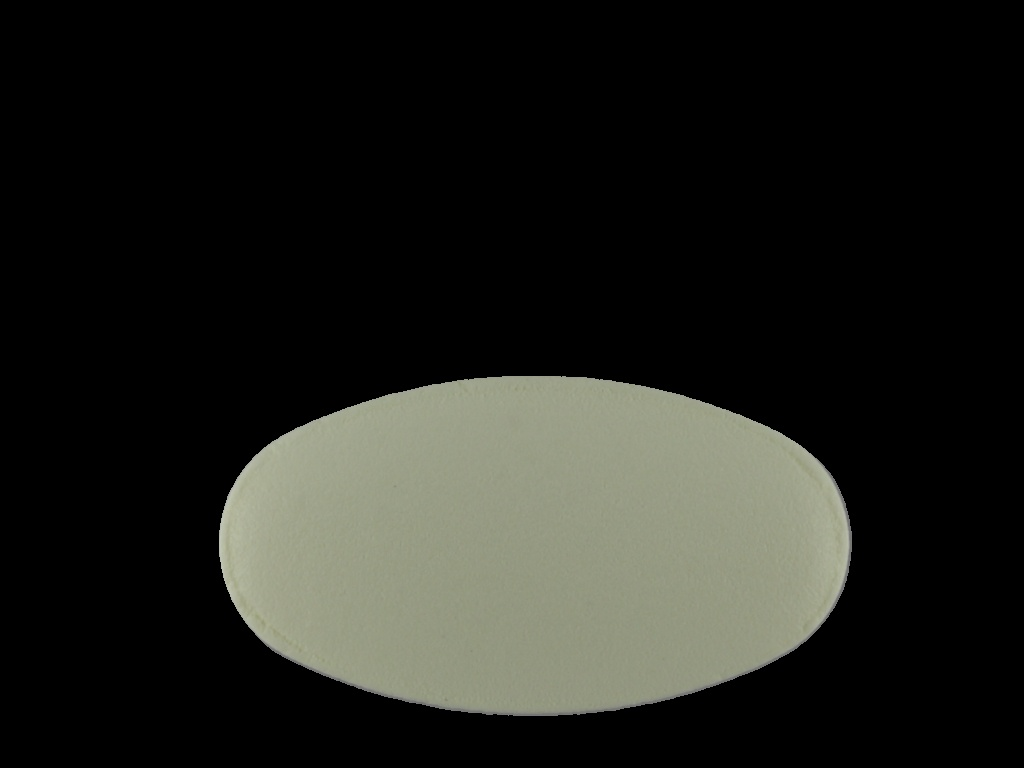
\includegraphics[width=0.25\textwidth]{figuras/eletronica/processamento/pilula2.jpg}\label{fig:proPill2}}
        
        \caption{Processo de separação}
        \label{fig:proCond}
\end{figure}

\subsection{Extração de características}

Com os comprimidos separados, é possível extrair informações que serão utilizadas para classificá-los.

\begin{itemize}
    \item \textbf{Cor}
    
    Para extrair a cor do comprimido, será utilizada uma média da cores de toda a região, eliminando possíveis efeitos de sombra presentes. Sendo assim, serão estabelecidos rótulos que corresponderão a uma faixa específica do espectro RGB das imagens.
    
    \item \textbf{Formato}
    
    Para extrair o formato do comprimido, será utilizada a técnica de \textit{template matching}. Ela consiste em comparar a imagem com modelos pré-definidos, realizando a correlação da imagem com o \textit{template}. Se a correlação for próxima de 1, significa que há uma alta probabilidade do formato estar correto. Consequentemente, é possível testar todos os formatos possíveis e identificar qual a maior correlação entre eles.
    
    \item \textbf{Texto estampado}
    
   O tratamento da imagem é necessário para extrair o texto do comprimido, para que os contornos sejam destacados. Com isso, obteremos a Fig. \ref{fig:propilLim}, apesar do objeto de texto ainda possuir áreas não conectadas. Para contornar esse problema, é utilizado uma abertura na imagem com um objeto estruturante circular pequeno com até 5 pixeis de diâmetro. Assim, obtemos como resultado uma melhor definição das letras, mostrada na Fig. \ref{fig:propilAb}.
    
    Por fim, subtrai-se a máscara do comprimido do resultado anteriormente obtido e, consequentemente, no isolamento do texto a ser processado. O resultado da subtração da máscara pode ser visualizado na Fig. \ref{fig:propiltext}.
    
    Para interpretar o texto, será utilizado o \textbf{Tesseract}, um sistema de reconhecimento óptico de caracteres (OCR), o qual utiliza uma rede neural treinada para identificar linhas de texto. Para utilização desse sistema, é necessário identificar a região de interesse e isolá-la para melhores resultados. Assim, obtemos o resultado na Fig. \ref{fig:propiltextex}, onde é possível observar a região de interesse que possui texto e o valor reconhecido.
    
    \begin{figure}[H]
        \centering
        \subfloat[][Destaque dos contornos]{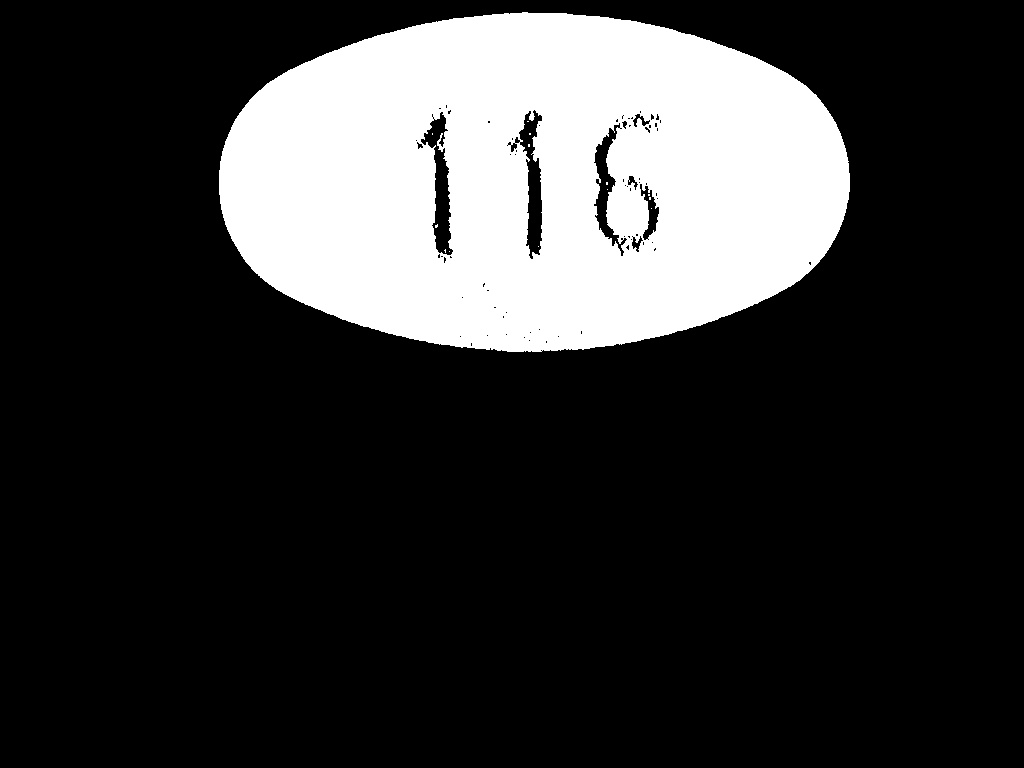
\includegraphics[width=0.3\textwidth]{figuras/eletronica/processamento/pilulalimiar.jpg}\label{fig:propilLim}}
        \hspace{0.05cm}
        \subfloat[][Conexão das letras]{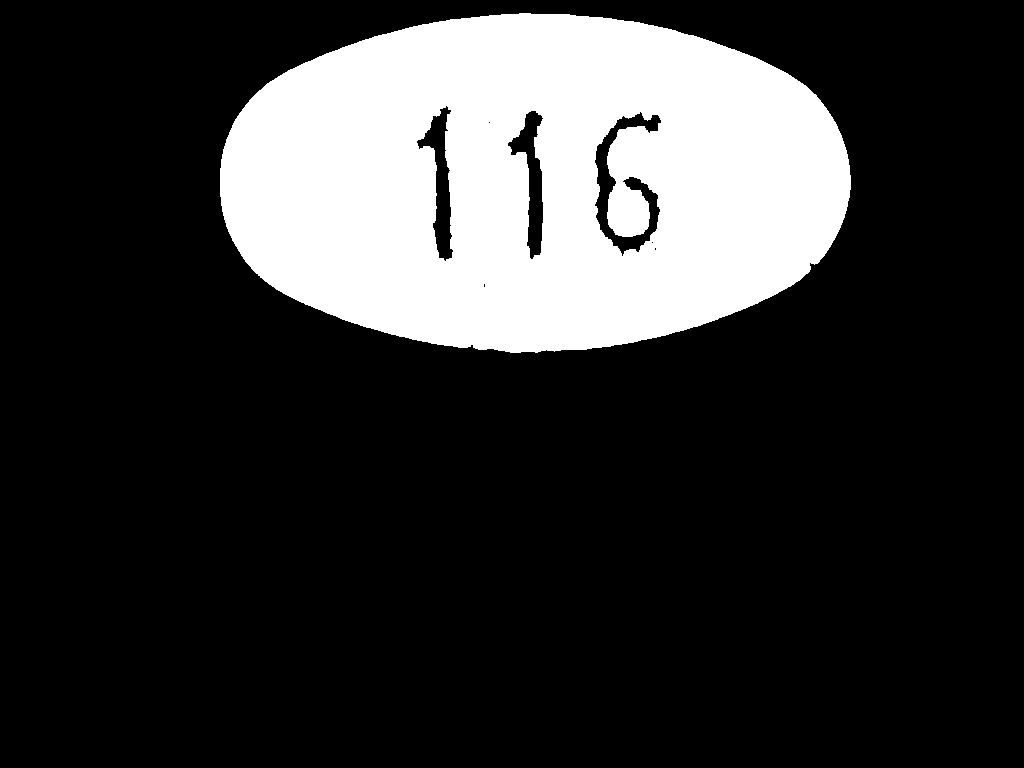
\includegraphics[width=0.3\textwidth]{figuras/eletronica/processamento/pilulaabertura.jpg}\label{fig:propilAb}}
        \hspace{0.05cm}
        \subfloat[][Texto isolado]{
\includegraphics[width=0.3\textwidth]{figuras/eletronica/processamento/texto.jpg}\label{fig:propiltext}}
        
        \subfloat[][Texto identificado]{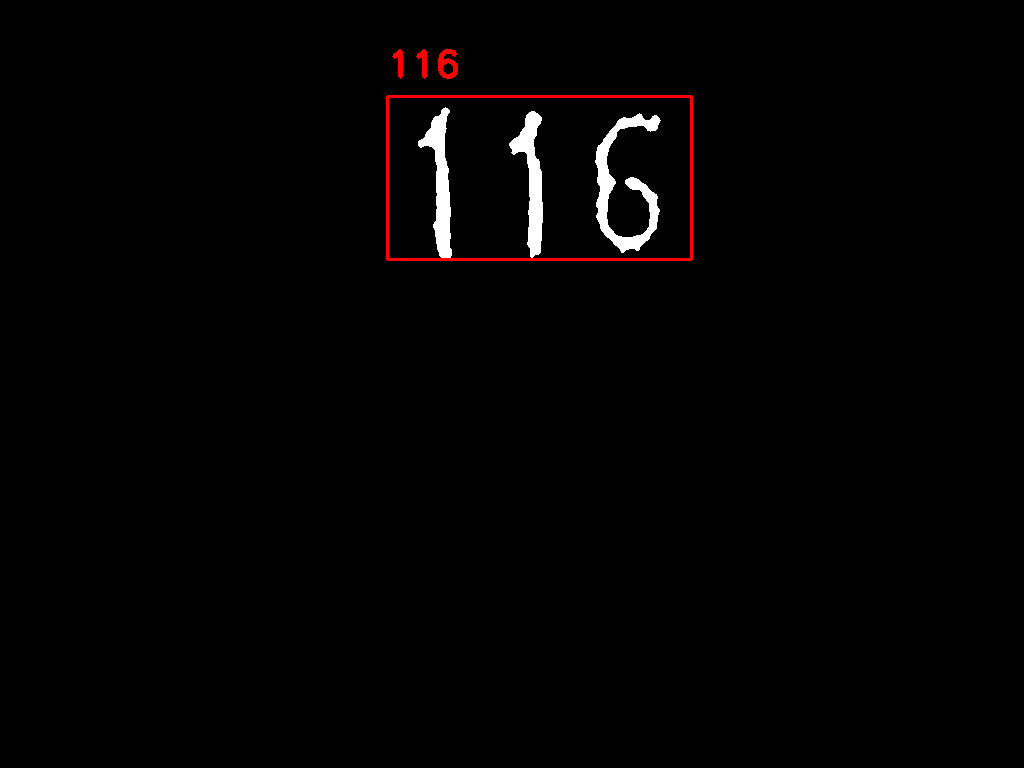
\includegraphics[width=0.4\textwidth]{figuras/eletronica/processamento/textoExtraido.png}\label{fig:propiltextex}}
        
        
        \caption{Extração de texto}
        \label{fig:proText}
    \end{figure}
\end{itemize}

\subsection{Máquina de Vetores de Suporte (SVM)}

Para conseguir identificar diversos comprimidos nas imagens, é necessário o uso de um classificador. Existem diversos tipos de classificadores, e o escolhido foi a máquina de vetores de suporte (SVM). 

Seu funcionamento se baseia na ideia de gerar uma superfície que separa as classificações por meio das características empregadas. Dessa forma, para realizar o treinamento da SVM, são criados vetores de suporte que separam a área entre classificações.

Assim, para o treinamento, será utilizado um banco de imagens de comprimidos feito pela \textit{National Library of Medicine} que possui 4 mil imagens em ambiente controlado e 133 mil imagens amadoras. O banco de imagens está disponível no  \href{https://www.nlm.nih.gov/databases/download/data_distrib_main.html}{link}. 

O tipo de classificação utilizada será a `\textit{yes or no}', na qual serão criadas SVMs para cada comprimido a ser identificado, e deve-se ensinar como identificar características individuais dos comprimidos.

